\documentclass[crop,tikz]{standalone}
\usetikzlibrary{calc}
\usetikzlibrary{arrows}
\usetikzlibrary{decorations.pathreplacing}
\begin{document}
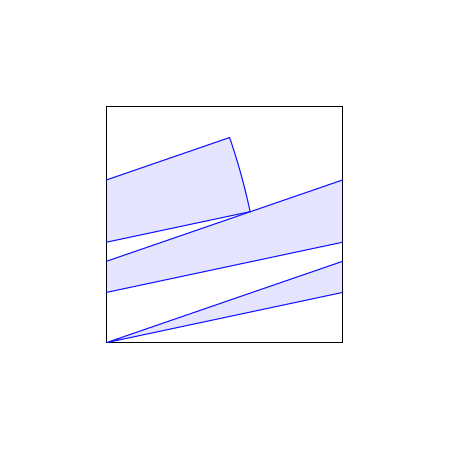
\begin{tikzpicture}
  % Constants
  \pgfmathsetmacro\b{3}
  \pgfmathsetmacro\d{8}
  \pgfmathsetmacro\t{7}
  \pgfmathsetmacro\a{12}
  % Boundary
  \path[use as bounding box] (0,0) rectangle (2+\b,2+\b);
  % Domain grids
  \draw (1,1) -- (1+\b,1) -- (1+\b,1+\b) -- (1,1+\b) -- cycle;
  % Lightcone
  \begin{scope}[shift={(1,1)}]
    \clip (0,0) rectangle(\b,\b);
    \filldraw[fill=blue,fill opacity=0.1,draw=blue!90] (0,0) -- (\a:\d) arc (\a:\a+\t:\d) -- cycle;
  \end{scope}
  \begin{scope}[shift={(1-\b,1)}]
    \clip (\b,0) rectangle(2*\b,\b);
    \filldraw[fill=blue,fill opacity=0.1,draw=blue!90] (0,0) -- (\a:\d) arc (\a:\a+\t:\d) -- cycle;
  \end{scope}
  \begin{scope}[shift={(1-2*\b,1)}]
    \clip (2*\b,0) rectangle(3*\b,\b);
    \filldraw[fill=blue,fill opacity=0.1,draw=blue!90] (0,0) -- (\a:\d) arc (\a:\a+\t:\d) -- cycle;
  \end{scope}
\end{tikzpicture}
\end{document}
